\section{Computational Methods}

Molecular dynamics simulations were performed using the Amber 11 software suite.\cite{Case2010} In this study we incorporate polarizable models for the \wat~and \suldiox~molecules. Fully polarizable models have been used previously in studies on interfacial systems because they are known to more accurately reproduce interfacial structure and free energy profiles.\cite{Wick2007,Rivera2006,Dang1998} The \wat~model used is the POL3 model,\cite{Caldwell1995} and for \suldiox we used the model of Dang, et al. that places a single polarizable center on the sulfur atom.\cite{Baer2010}

All simulations began with an equilibrated cube of 900 \wat~molecules, with sides of length 30\angs. The simulations all employed periodic boundaries to create an ``infinite-slab'' geometry for the water phase. One set of simulations involved adding a single \suldiox~to the center of the water box and then allowing the system to equilibrate over 1 ns of simulation. The system was then evolved for a further 2.5 ns with atomic coordinates written every 100 fs. The simulation is herein referred to as the ``surface equilibrated'' simulations. 

\subsection{Steered Molecular Dynamics}

A second set of simulations involved preparing an equilibrated water slab as in the surface equilibrated method. A single \suldiox~was then introduced 20\angs above the slab, with the sulfur atom tethered to its initial position. The system was evolved for 1 ns, taking coordinate snapshots every 20 ps to create 50 starting points for further simulations. Steered molecular dynamics (SMD) were then performed to guide the \suldiox~down towards a tethered water 15\angs under the water slab surface by applying a small steering force.\cite{Isralewitz2001} The \suldiox~thus passed through the continuum of environments from gas phase to hydrate complex interaction, water surface adsorption, and absorption into the bulk of the neat-\wat~slab.

The third set of simulations were performed similarly to the neat-\wat~and single \suldiox~SMD simulations, but the water slab and gas phase above it were first saturated with \suldiox. The water slab was loaded internally with 22 \suldiox molecules, which represent a saturation level coinciding with the Henry's law constant for \suldiox~in \wat. The gas phase was populated with 50 \suldiox~molecules representing approx. 50 atm of \suldiox~pressure. As in the neat-\wat~SMD simulations, a single \suldiox~was introduced 20\angs above the saturated water slab surface and then steered into the bulk of the water. Figure \ref{fig:starting-configurations} illustrates two sample starting configurations for the SMD simulations, showing both the neat-\wat~slab and the saturated-\wat~slab configurations before steering the \suldiox~into the water bulk.

\begin{figure}[h!]
	\begin{center}
		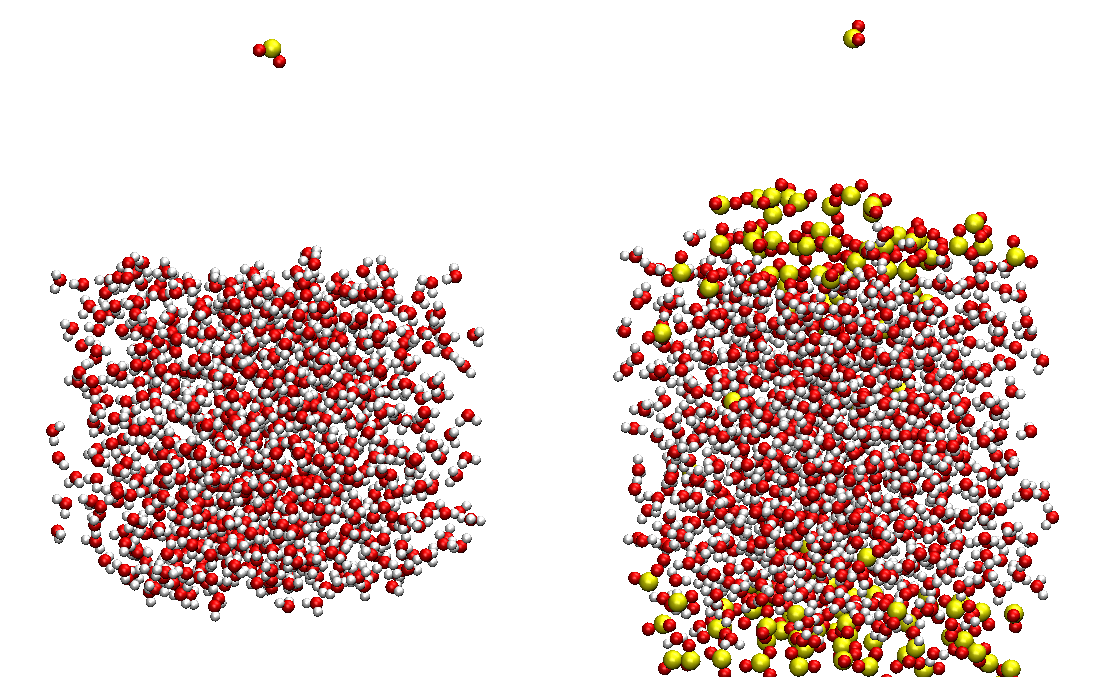
\includegraphics[scale=1.0]{images/startingconfigurations.png}
		\caption{Sample starting configurations for the two types of SMD simulations. The neat-\wat~slab simulation introduces a single \suldiox~molecule that is then guided into the surface of the water and further into the bulk (left). The saturated-\wat~slab simulation begins with different configurations of a water system that has been loaded with \suldiox~to saturate the water phase, and also with a high pressure of \suldiox~gas (right). The single \suldiox~(shown at the top) is then steered through the surface region saturated with \suldiox~molecules, and into the water bulk.}
		\label{fig:starting-configurations}
	\end{center}
\end{figure}
